% Slides 5--10: data, inherited framework, and precipitation development.

\begin{frame}{Sixteen years of building-level insurance data}
  \begin{columns}[T,onlytextwidth]
    \begin{column}{0.40\textwidth}
      \textbf{The data come from Gjensidige}
      \begin{itemize}
        \item One of Norway's largest insurers, with roughly a quarter of
          the market
        \item We have modelled their pluvial water damages for years, and
          published an article on the previous model
        \item This project is a three-way collaboration: Gjensidige, NR
          and ECoCA
      \end{itemize}

      \vspace{0.3cm}
      Building portfolio, 2010--2025:
      \begin{itemize}
        \item Daily claim timing and building-level exposure
        \item Claims, payouts, deductibles and claim-free periods
        \item Several residential and commercial building types
        \item Values inflation adjusted to 2026 NOK
        % \item Claims below the deductible are not observed
      \end{itemize}
    \end{column}
    % \begin{column}{0.57\textwidth}
    %   % Replace with the English-labelled plot using the same filename.
    %   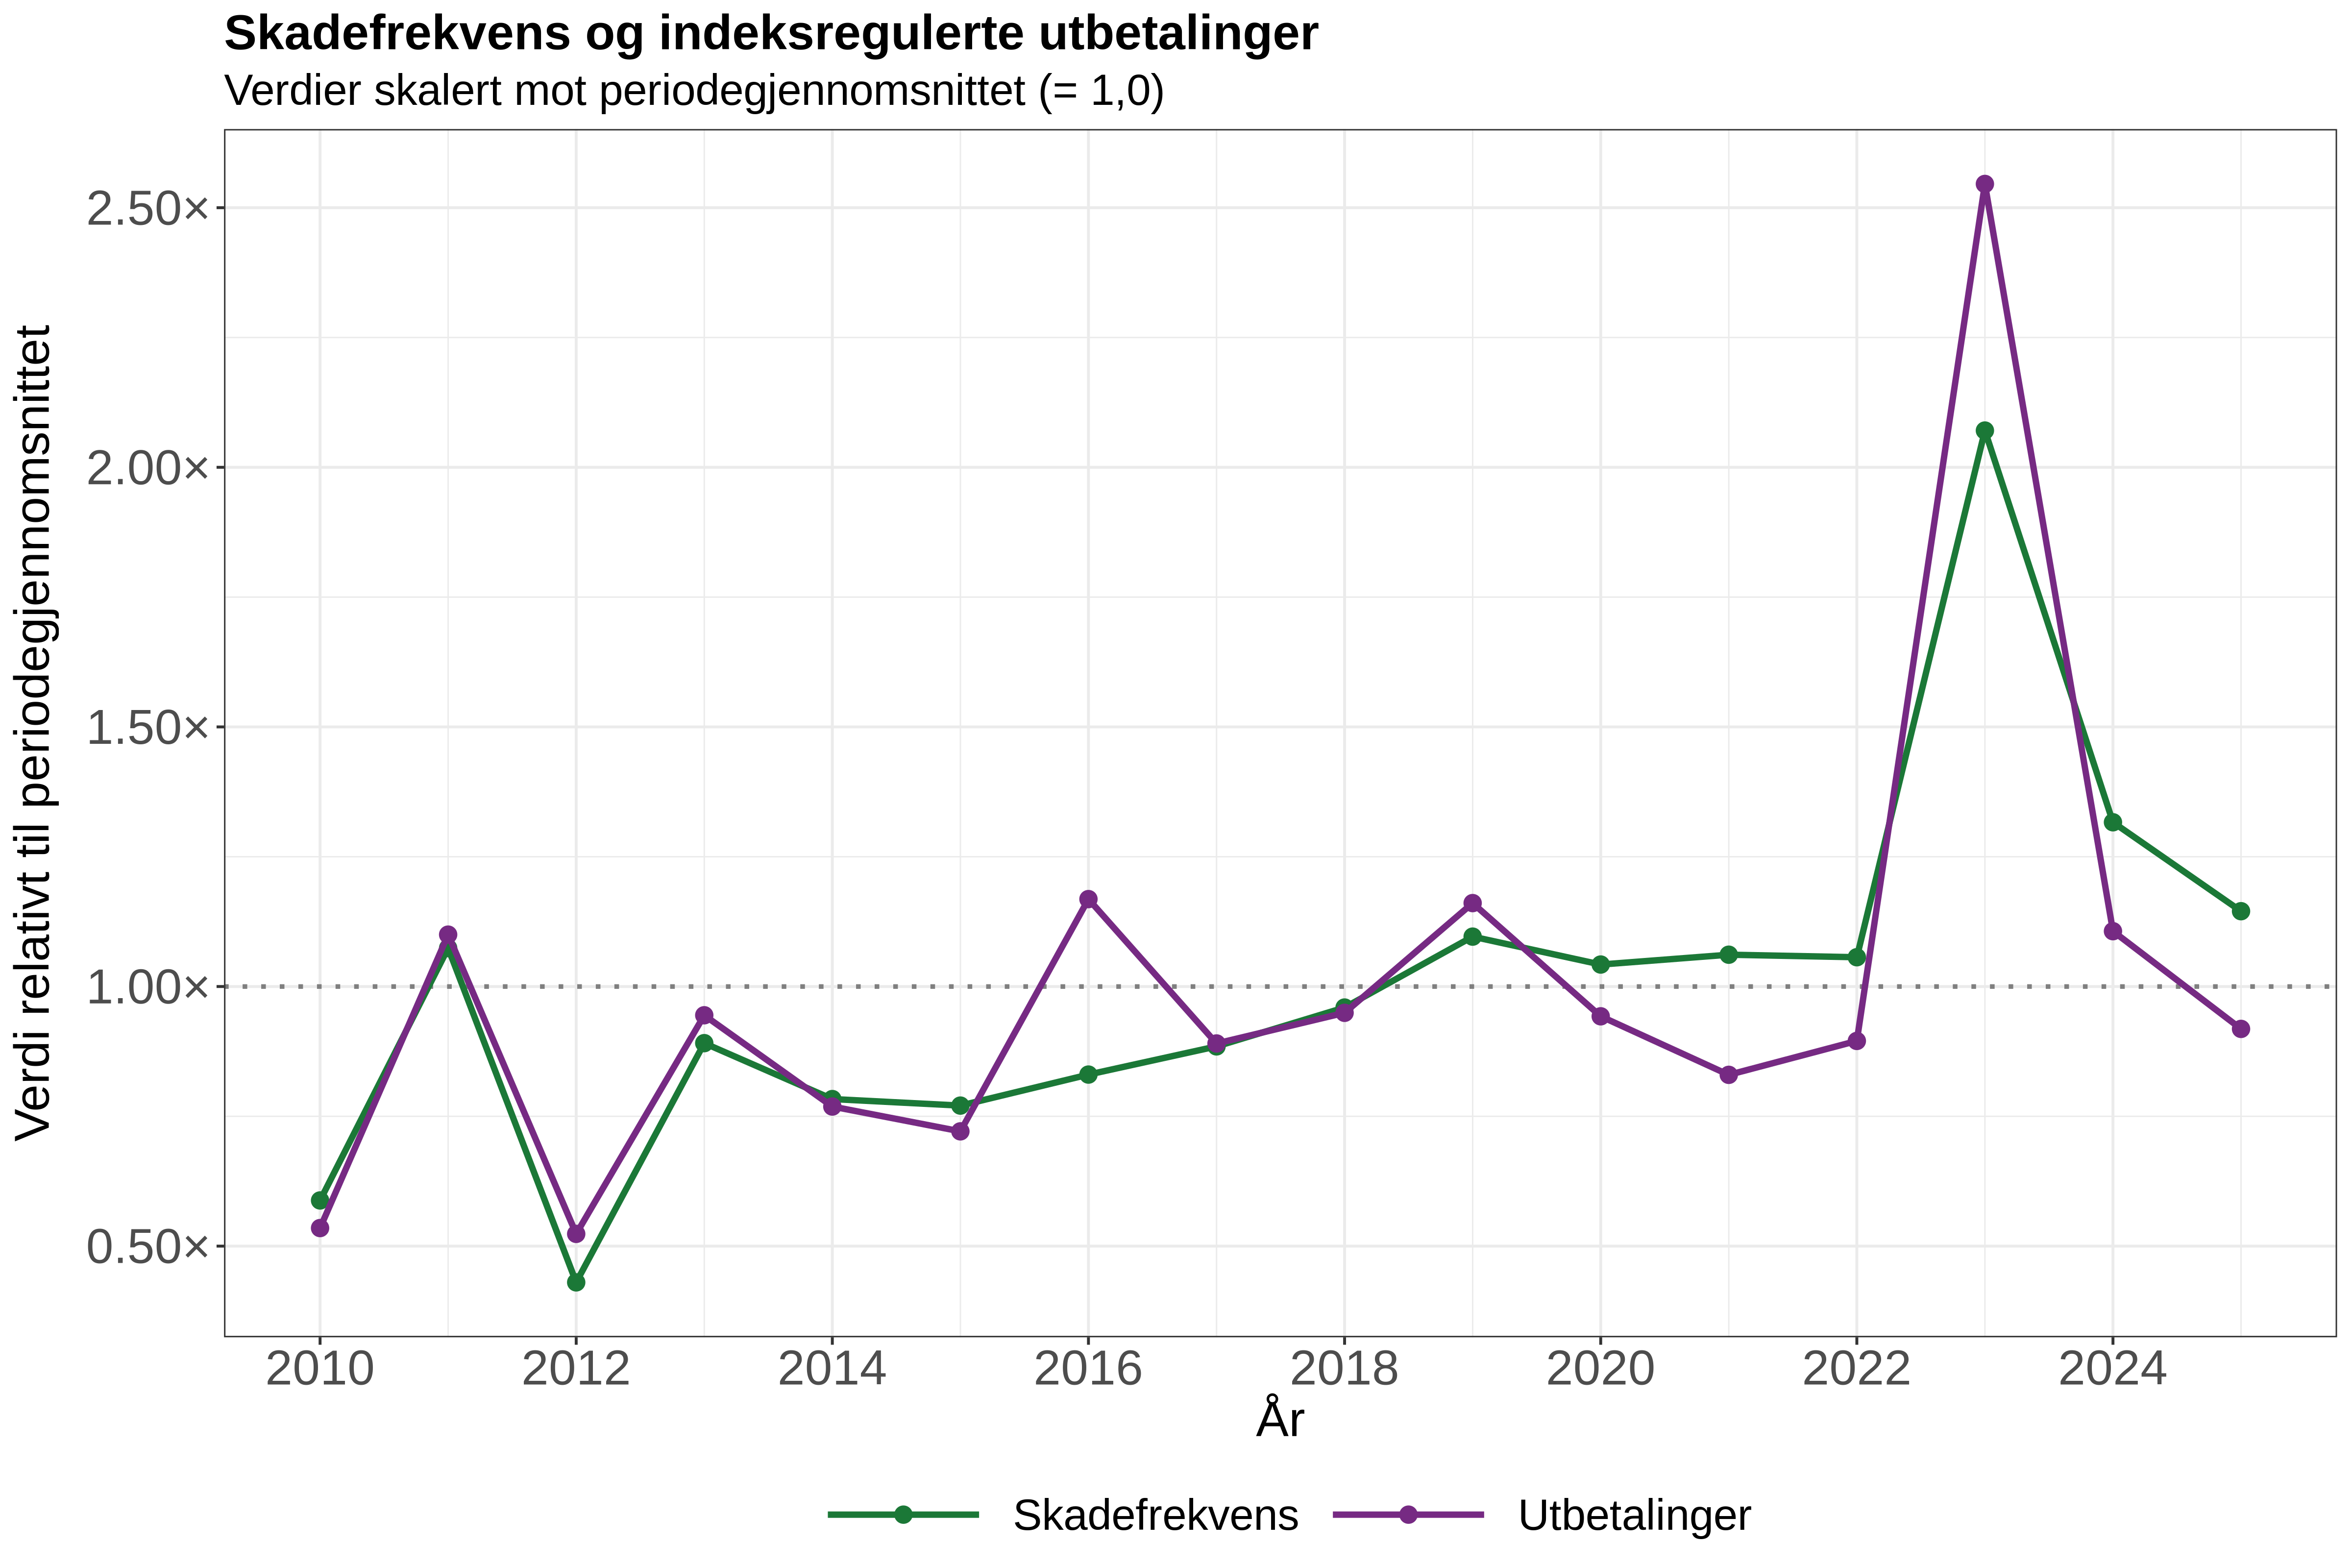
\includegraphics[width=\linewidth,height=0.60\textheight,keepaspectratio]{images/historical-claims.png}
    % \end{column}
  \end{columns}
  \sourceNote{Gjensidige building portfolio, 2010--2025}
\end{frame}

\begin{frame}{Weather, terrain and the built environment}
  \begin{columns}[T,onlytextwidth]
    \begin{column}{0.52\textwidth}
      \begin{itemize}
        \item \textbf{Weather:} daily seNorge precipitation and
          temperature on a 1 km grid
        \item \textbf{Terrain:} topographic wetness index and height
          above nearest drainage
        \item \textbf{Surface:} built-up versus non-built-up AR50 class
        \item \textbf{Building:} type, age, insured value, basement,
          standard and use
        \item \textbf{Region:} municipality and county effects
      \end{itemize}
    \end{column}
    \begin{column}{0.43\textwidth}
      \textbf{Modelling unit}

      One insured building in one year-season, linked to:
      \begin{itemize}
        \item local daily weather,
        \item fixed site characteristics, and
        \item the current insurance contract.
      \end{itemize}
    \end{column}
  \end{columns}
  \sourceNote{seNorge; Kartverket; NIBIO AR50; Gjensidige}
\end{frame}

\begin{frame}{We build on an existing risk model}
  \begin{columns}[T,onlytextwidth]
    \begin{column}{0.49\textwidth}
      \textbf{Retained from earlier work}
      \begin{itemize}
        \item Generalised additive models
        \item Separate frequency and severity models
        \item Building and topographic predictors
        \item Regional effects
      \end{itemize}
    \end{column}
    \begin{column}{0.47\textwidth}
      \textbf{Revised or new}
      \begin{itemize}
        \item Year-season precipitation indices
        \item Explicit focus on short-duration rainfall
        \item Updated 2024 regional structure
        \item Municipality-specific urban/rural effects
      \end{itemize}
    \end{column}
  \end{columns}
  \sourceNote{Heinrich and Mertsching (2023); current model development}
\end{frame}

\begin{frame}{Total cost = how often $\times$ how costly}
  \begin{columns}[T,onlytextwidth]
    \begin{column}{0.53\textwidth}
      \begin{itemize}
        \item \textbf{Claim frequency:} negative-binomial GAM for
          claims per insured exposure day
        \item \textbf{Cost per claim:} gamma GAM for payout
          conditional on a claim
        \item Both models use building, terrain, regional and
          precipitation covariates
        \item Simulated counts and severities are summed over
          buildings and seasons
      \end{itemize}
    \end{column}
    \begin{column}{0.42\textwidth}
      \vspace{0.7cm}
      \begin{align*}
        \text{total cost}
        &= \sum_{i,Q}\sum_{k=1}^{N_{iQ}}
        \left(A_i + U_{iQ}^{k}\right),\\[0.4cm]
        N_{iQ} &\sim \operatorname{NegBin},\\
        U_{iQ}^{k} &\sim \operatorname{Gamma}.
      \end{align*}
    \end{column}
  \end{columns}
  \sourceNote{Frequency--severity model for aggregate damage cost}
\end{frame}

\begin{frame}{Two precipitation indices survived validation}
  \begin{columns}[T,onlytextwidth]
    \begin{column}{0.53\textwidth}
      \begin{enumerate}
        \item \textbf{Absolute intensity}
          \begin{itemize}
            \item Mean precipitation across the three wettest days in
              a year-season
          \end{itemize}
        \item \textbf{Relative anomaly}
          \begin{itemize}
            \item Extreme-season rainfall relative to the local 95th
              percentile of daily precipitation
          \end{itemize}
      \end{enumerate}
    \end{column}
    \begin{column}{0.42\textwidth}
      \textbf{Interpretation}
      \begin{itemize}
        \item Damage requires sufficient water in absolute terms
        \item Local adaptation makes departures from normal
          conditions informative
      \end{itemize}

      Candidate indices were evaluated on unseen observations.
    \end{column}
  \end{columns}
  \sourceNote{Precipitation-index selection in the frequency model}
\end{frame}

% \begin{frame}{The same rainfall can mean different risk}
%   \begin{columns}[T,onlytextwidth]
%     \begin{column}{0.38\textwidth}
%       \begin{itemize}
%         \item Dry-climate locations respond more steeply than
%           wet-climate locations
%         \item At 40 mm, expected frequency is about nine times the
%           dry-season reference in the driest context
%         \item The comparable increase is about threefold in wetter contexts
%         \item Effects on cost per claim are smaller
%       \end{itemize}
%     \end{column}
%     \begin{column}{0.59\textwidth}
%       % Replace with English-labelled plots using the same filenames.
%       \centering
%       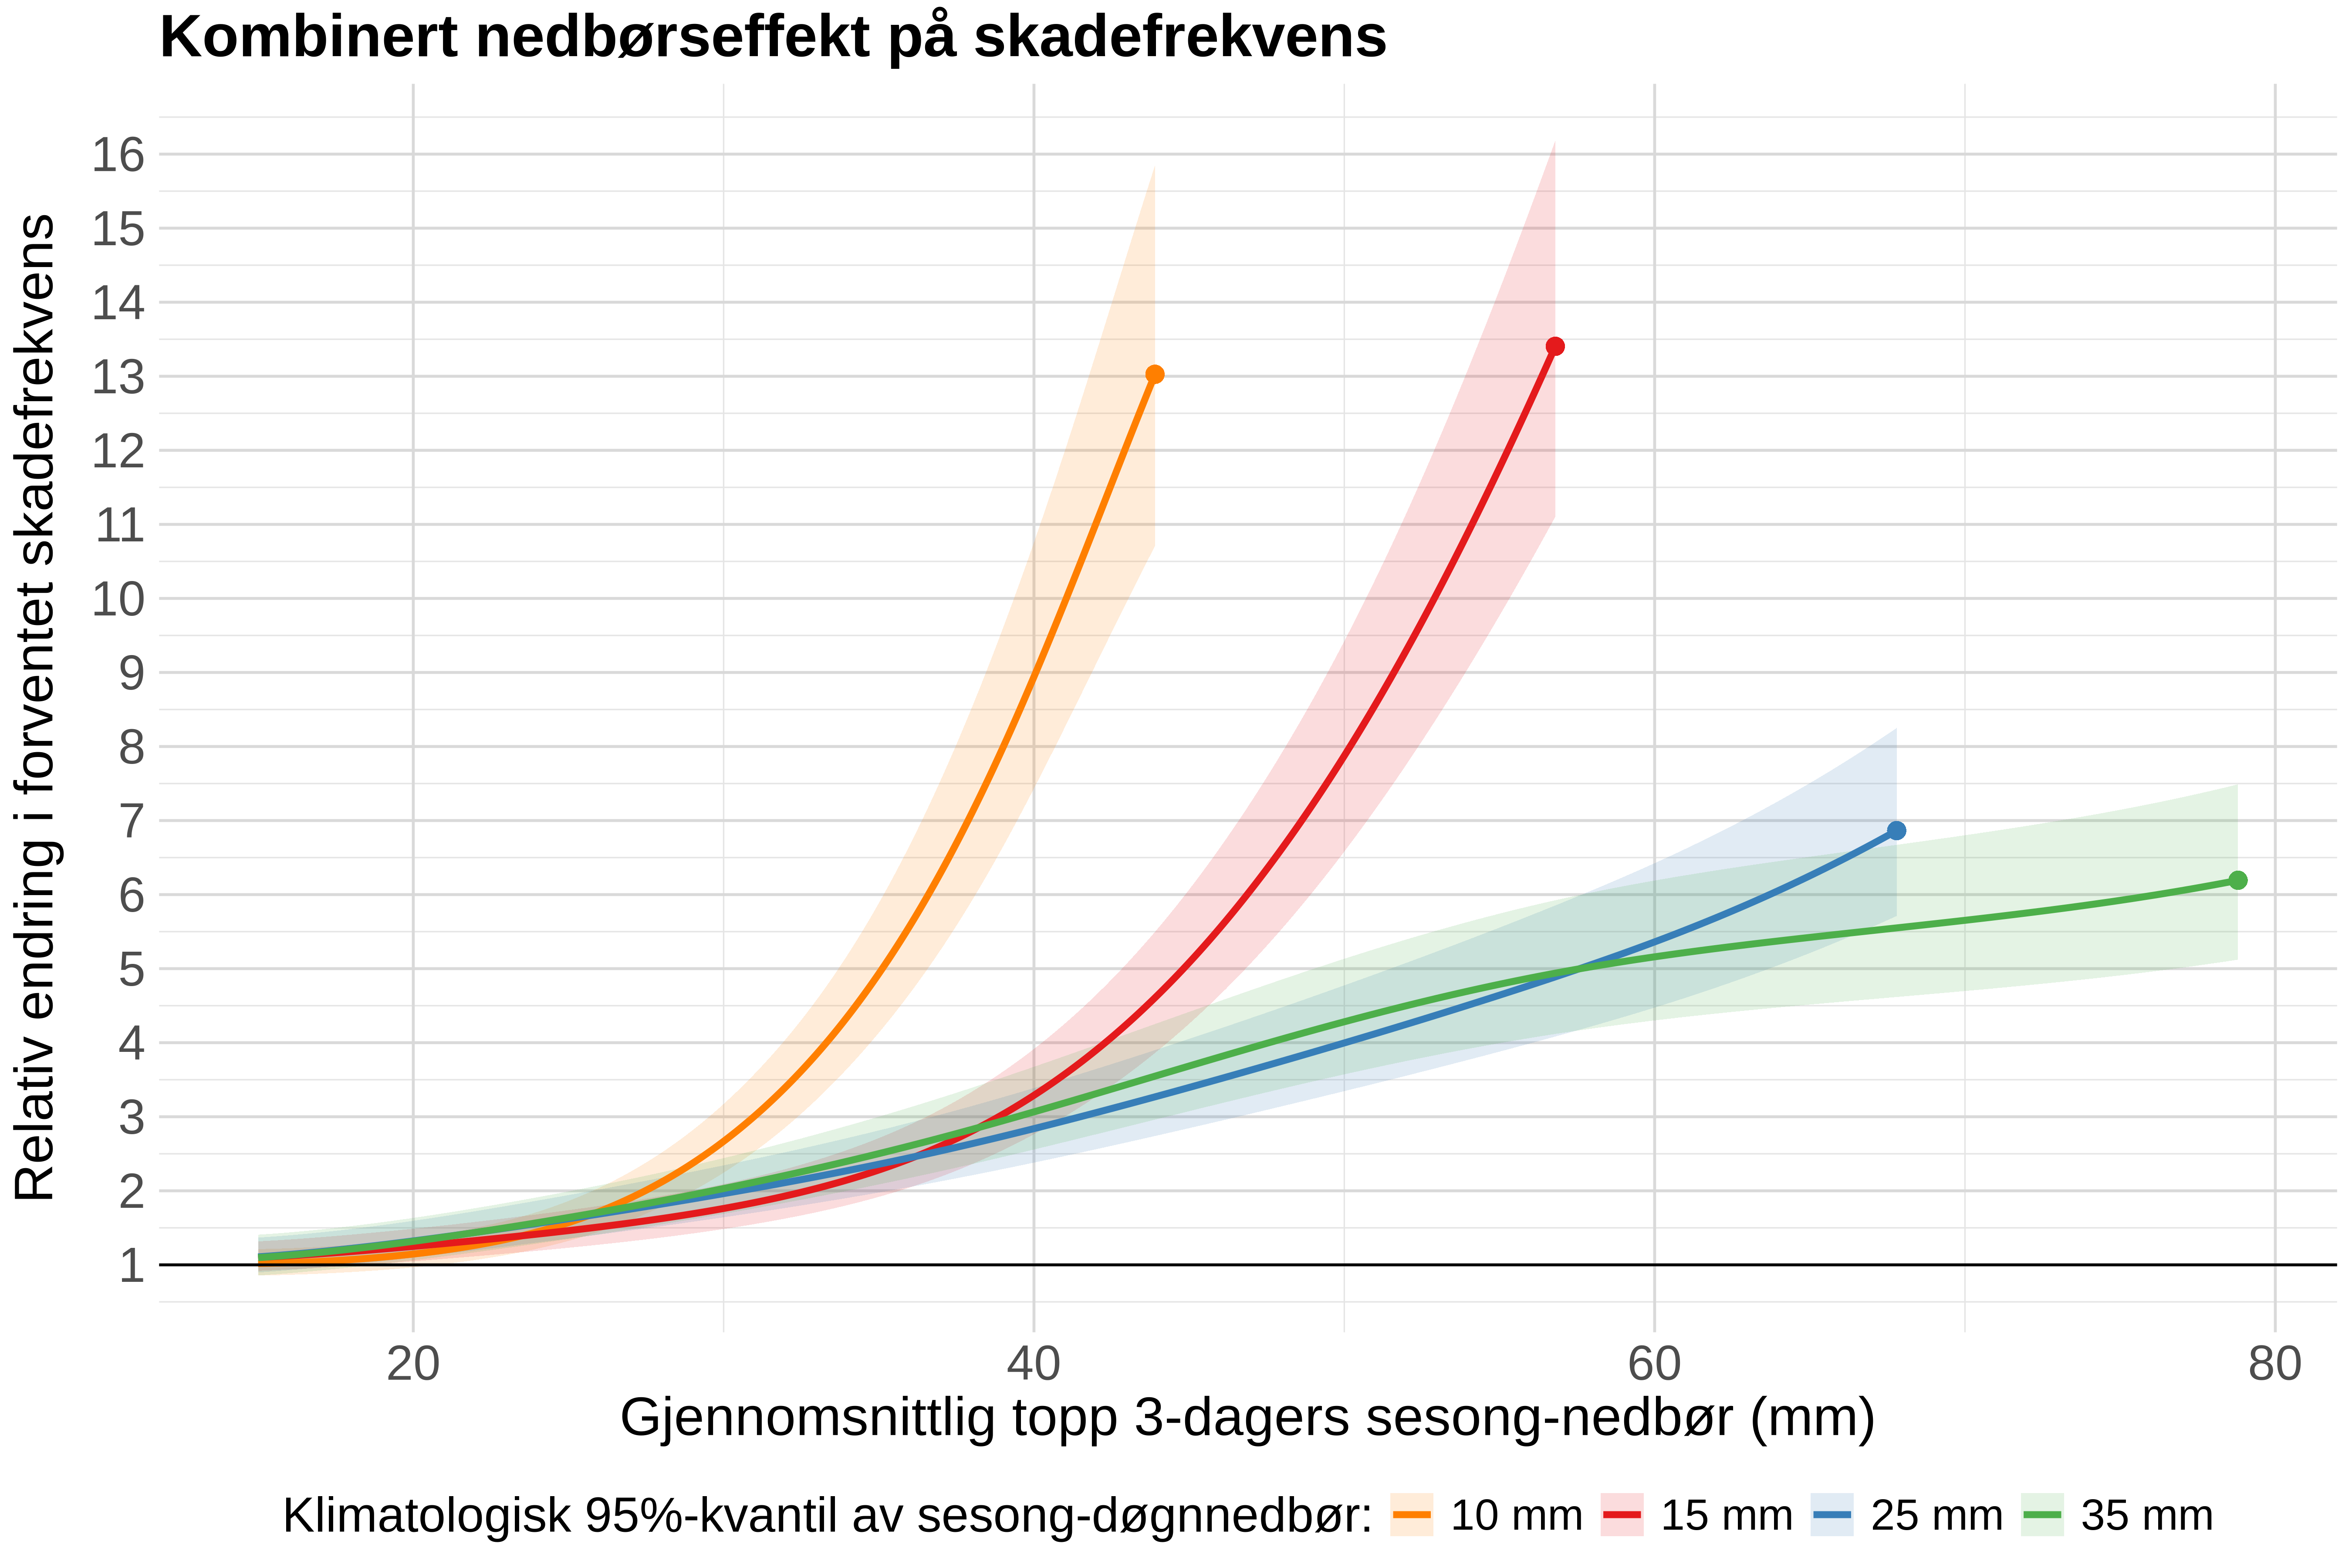
\includegraphics[width=0.88\linewidth,height=0.27\textheight,keepaspectratio]{images/precipitation-frequency.png}\\[-0.05cm]
%       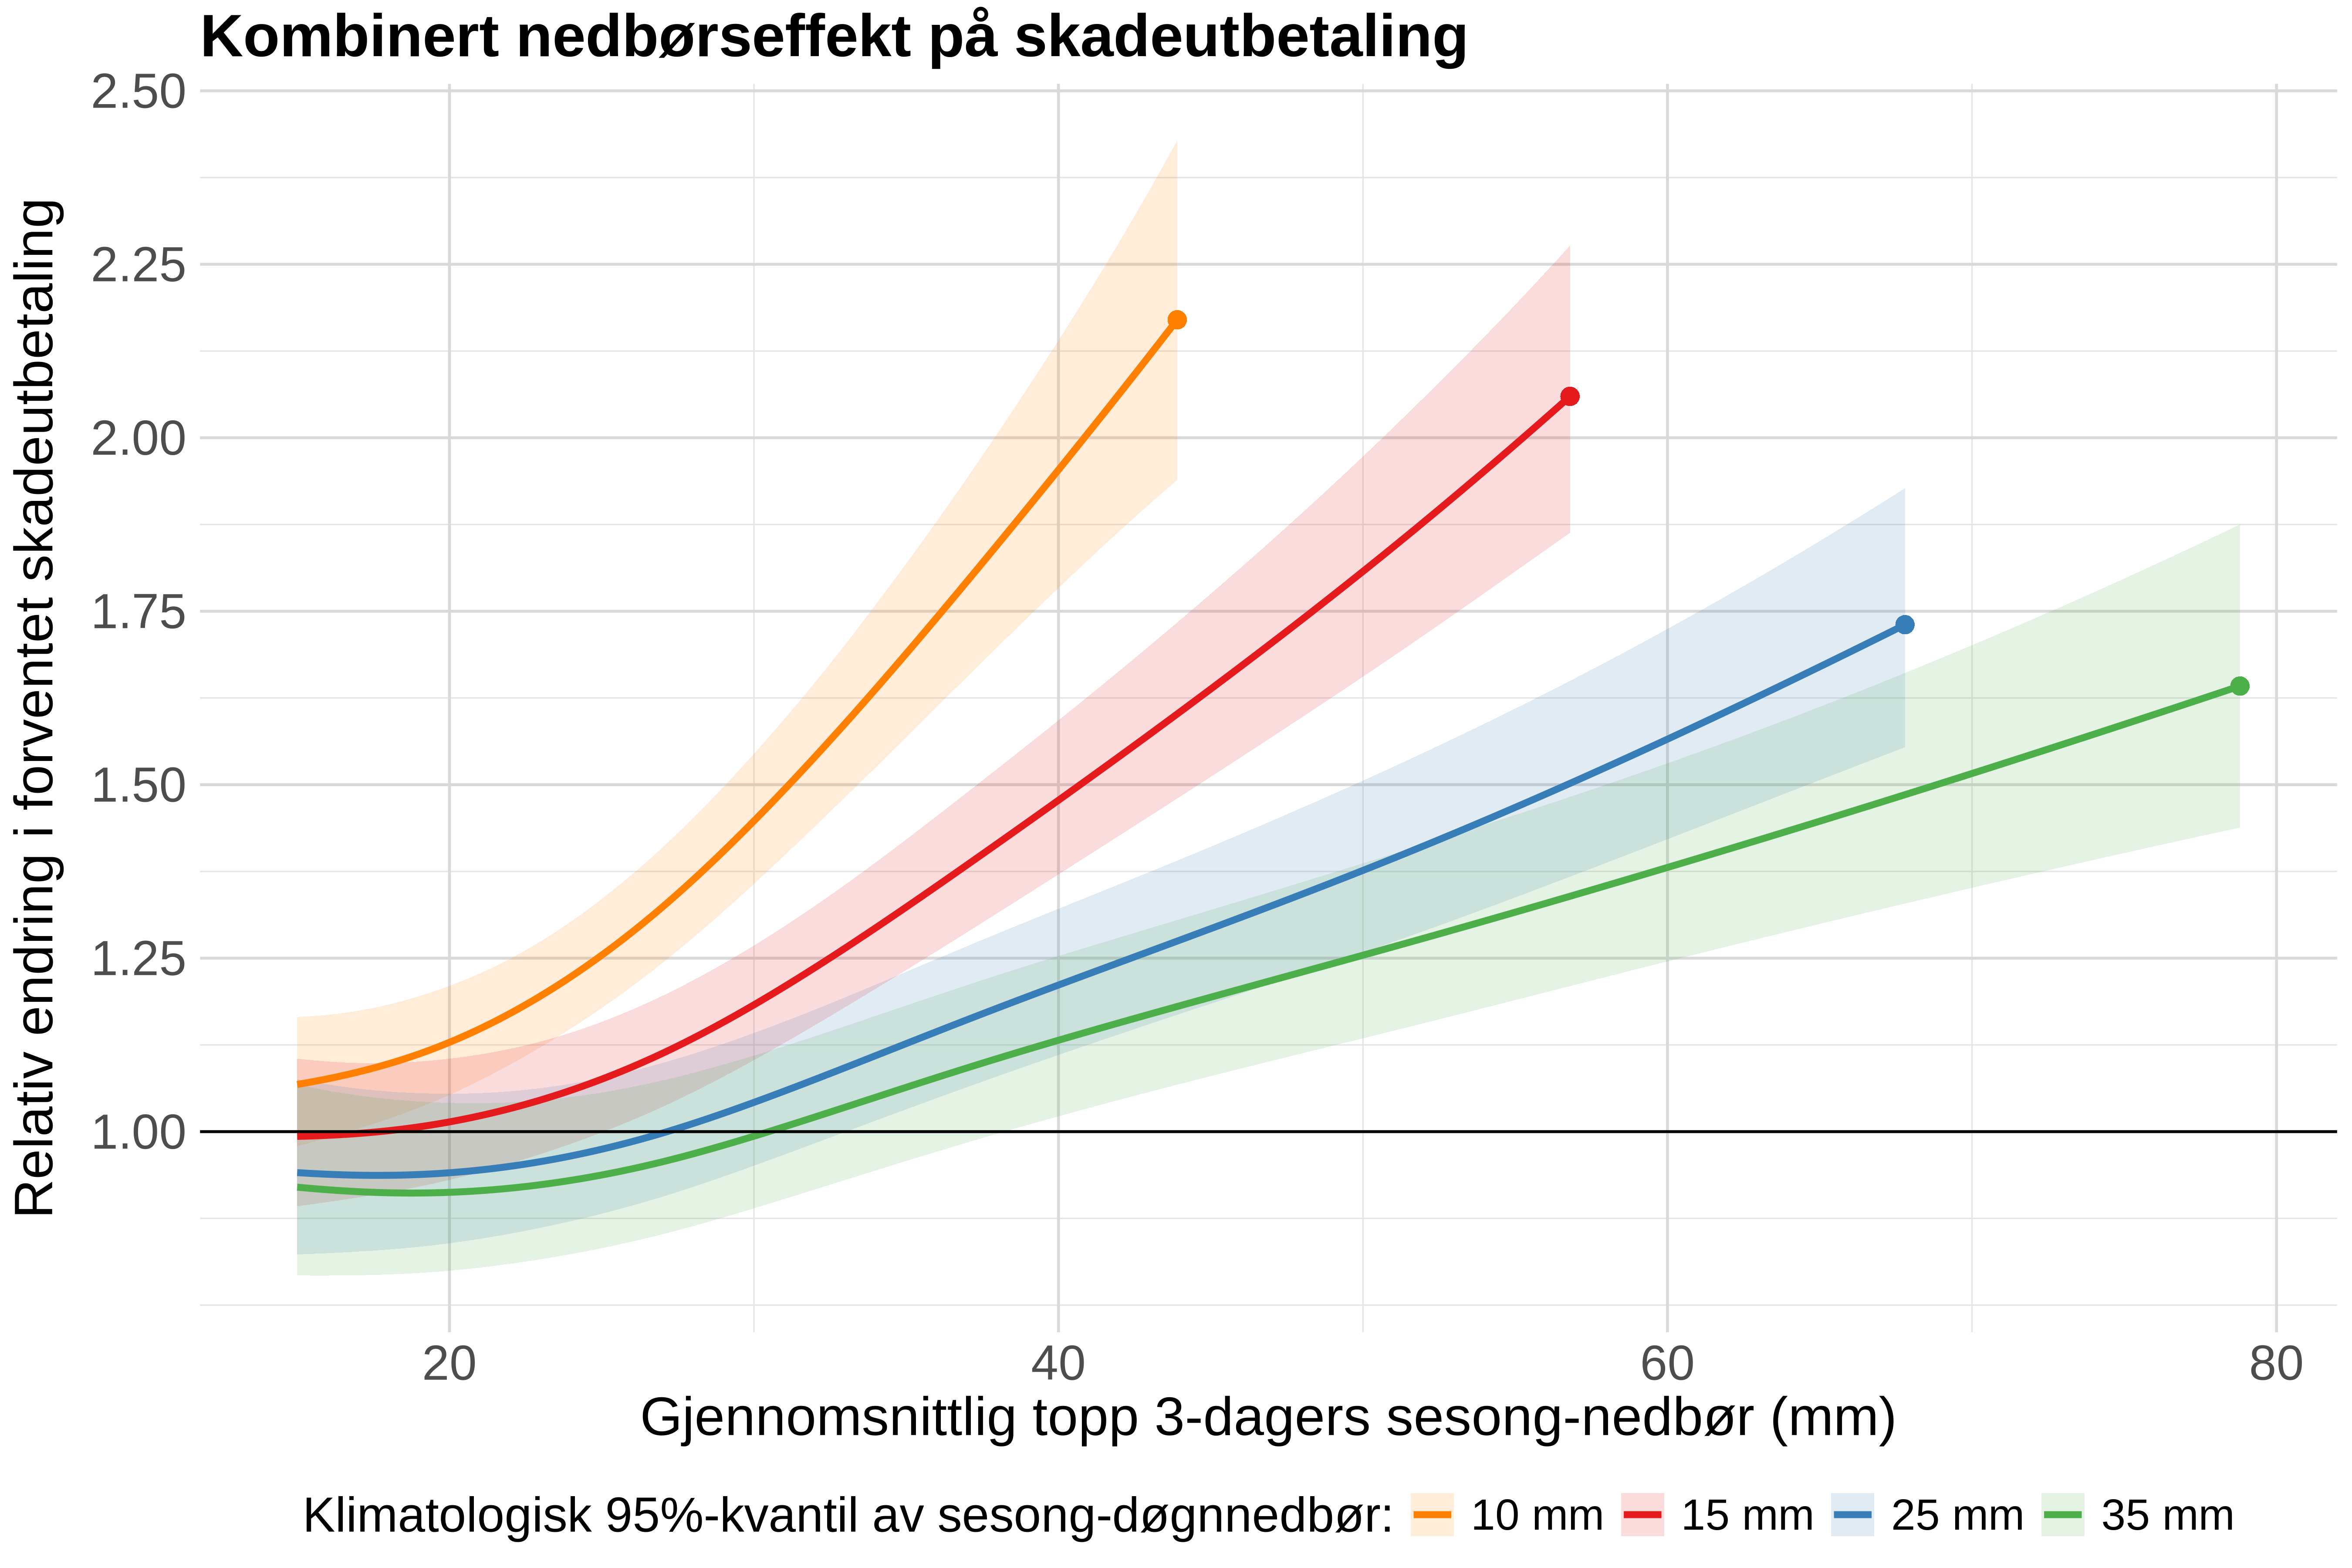
\includegraphics[width=0.88\linewidth,height=0.27\textheight,keepaspectratio]{images/precipitation-severity.png}
%     \end{column}
%   \end{columns}
%   \sourceNote{Combined marginal precipitation effects from the fitted models}
% \end{frame}

\begin{frame}{Precipitation effect on claim frequency}
  \centering
  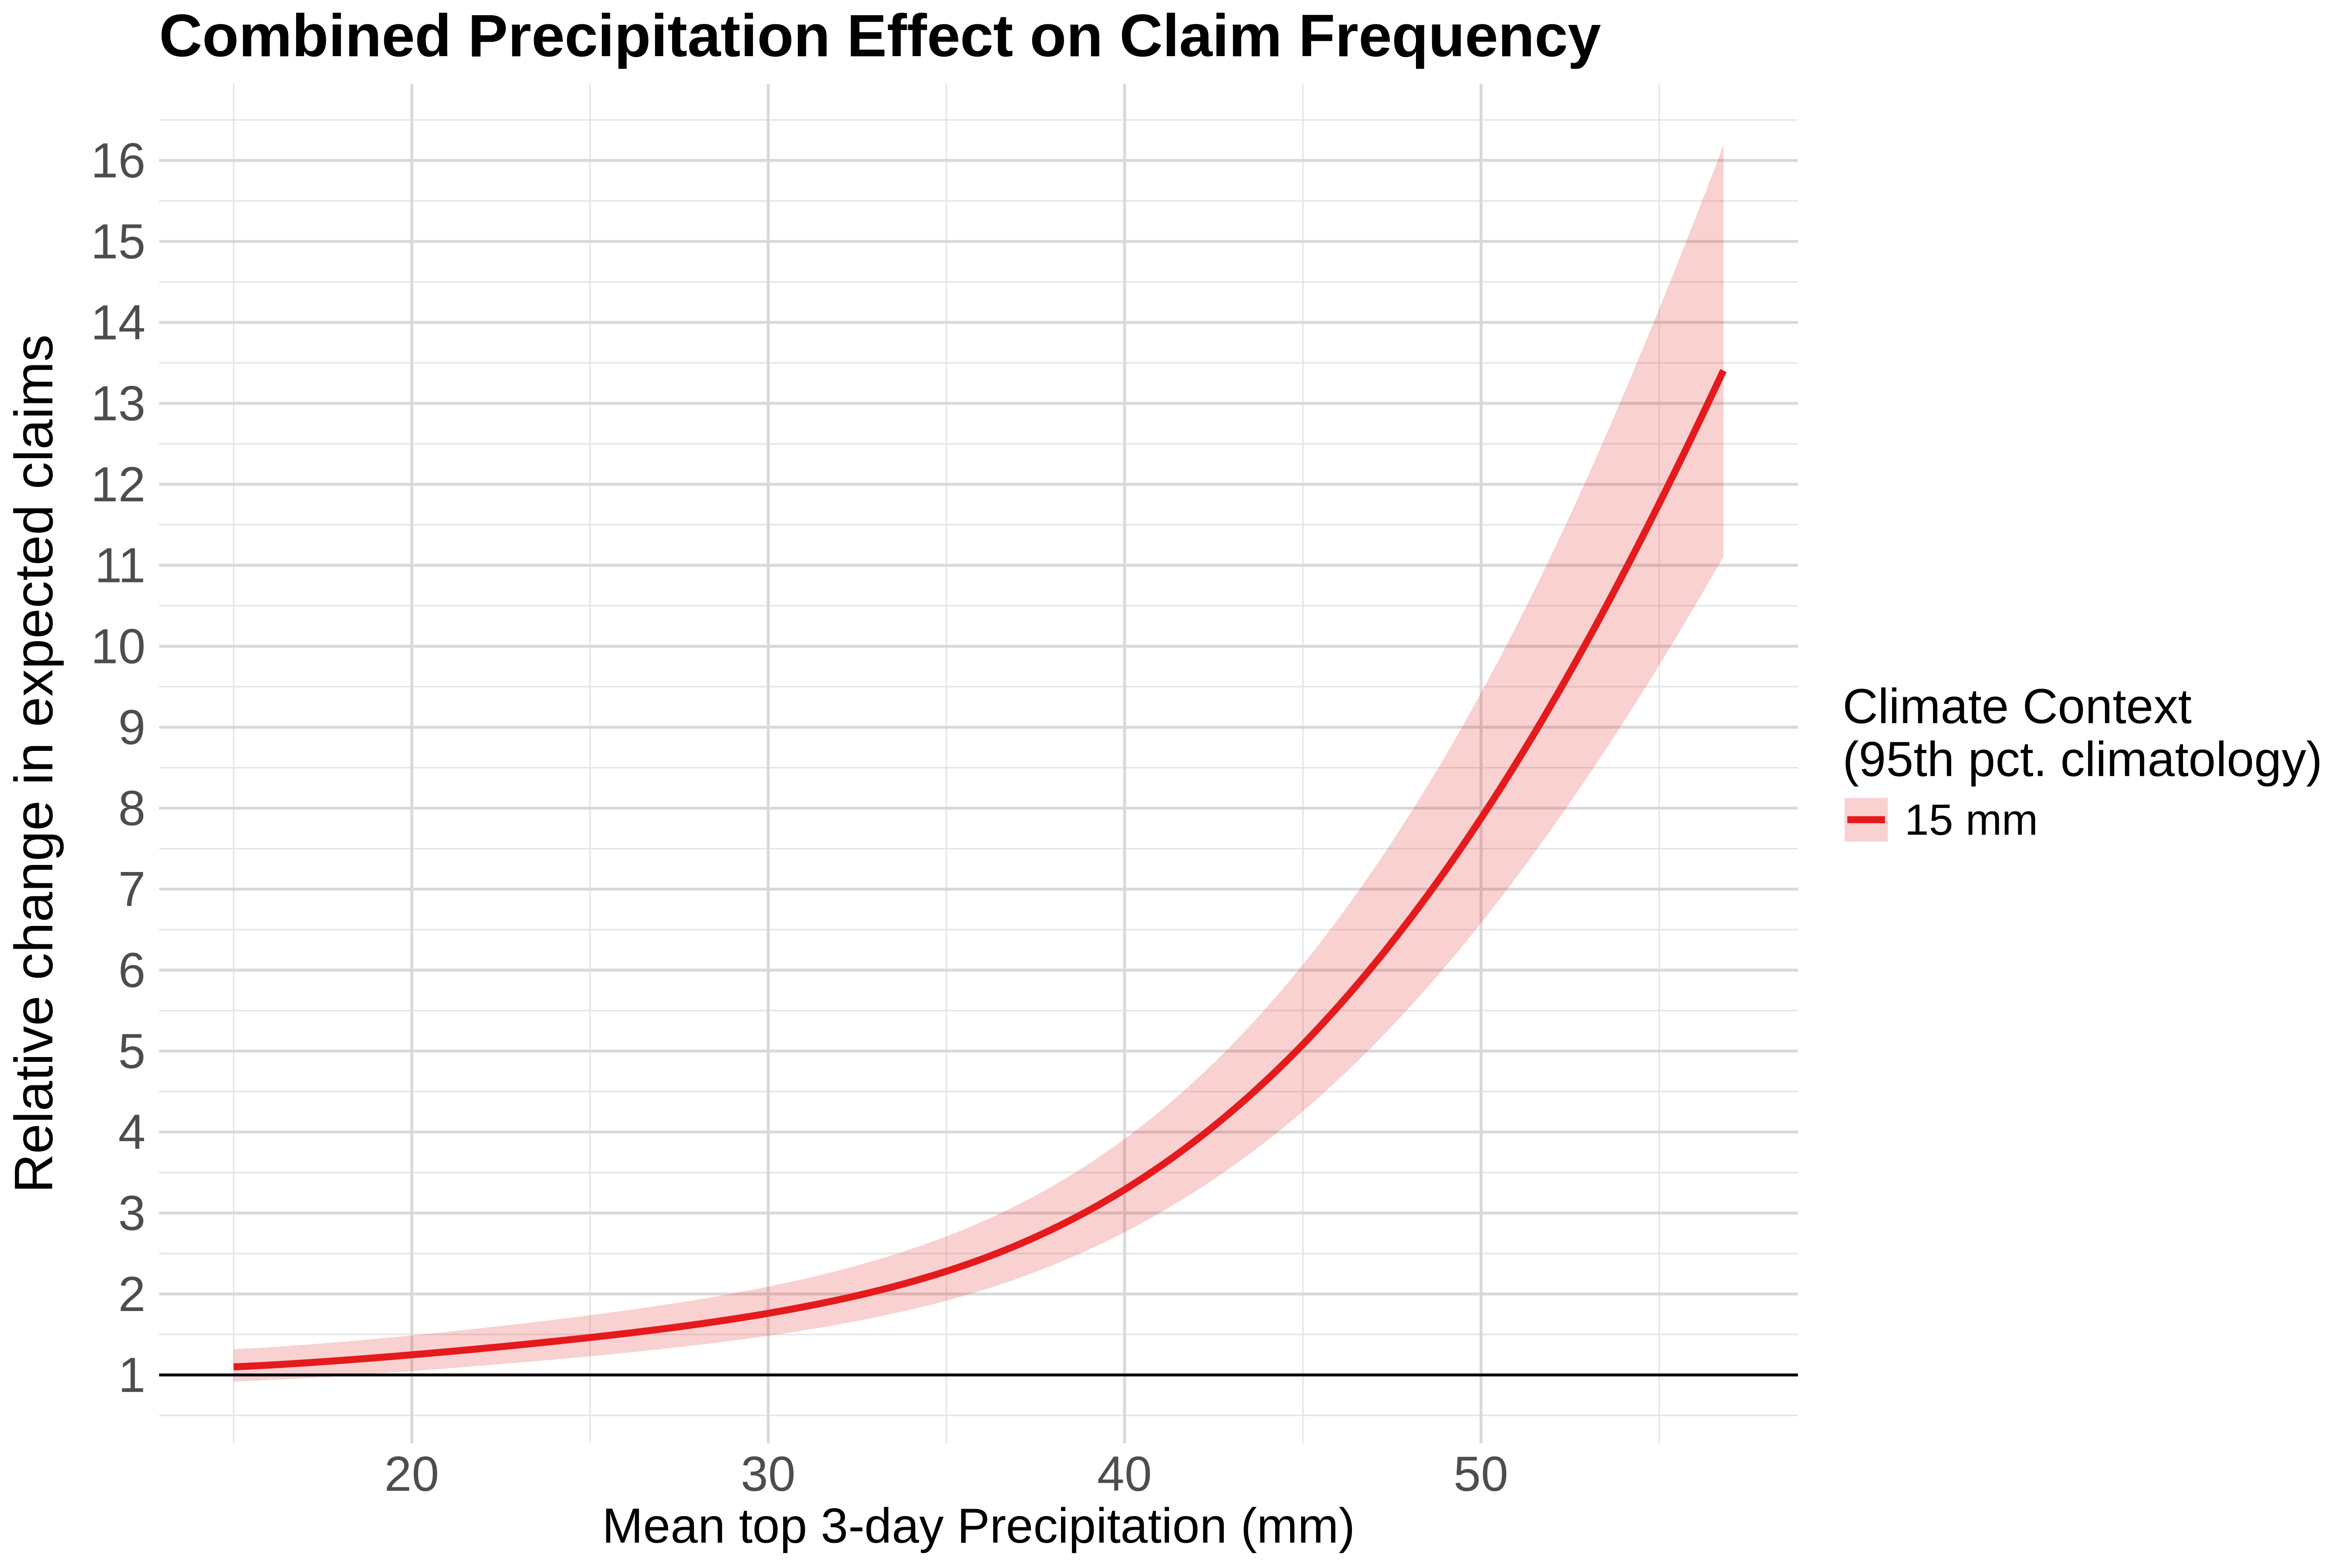
\includegraphics[width=\textwidth,height=0.75\textheight,keepaspectratio,trim={0
  0 0 26},clip]{
  images/model_effects/claim_incidence_combined_precipitation_effect_simple_presentation.png}
\end{frame}

\begin{frame}{Precipitation effect on claim frequency}
  \centering
  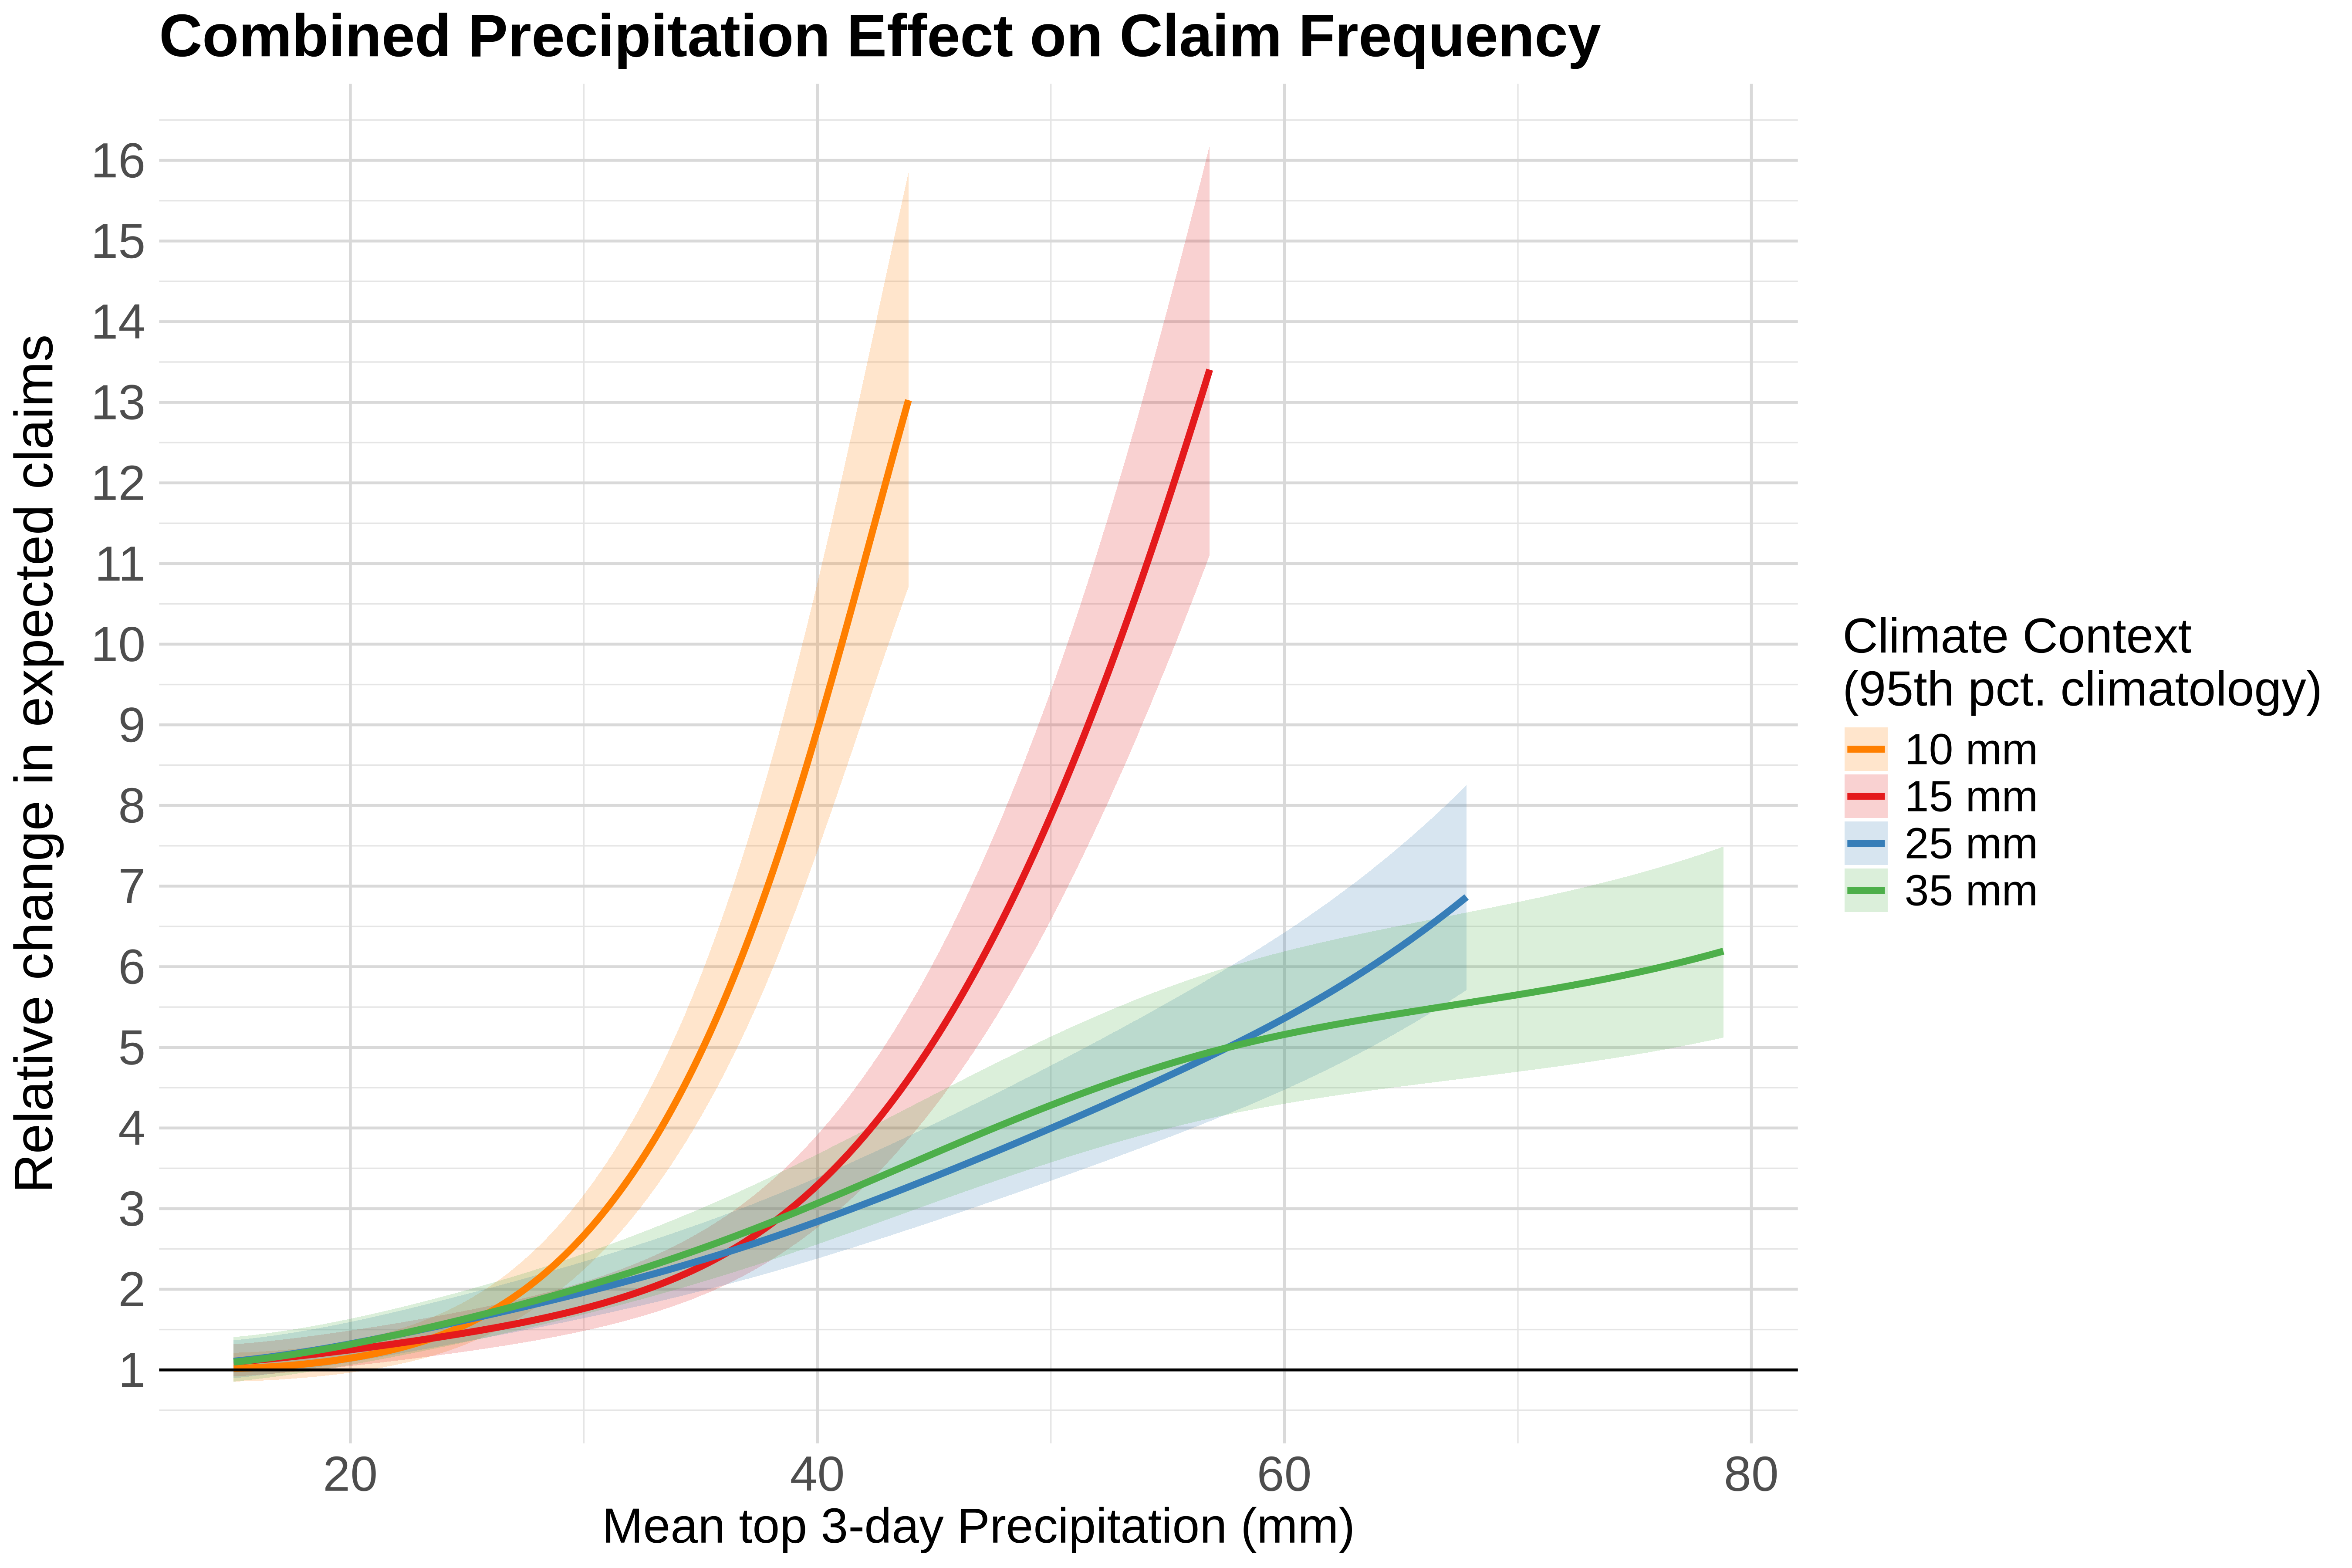
\includegraphics[width=\textwidth,height=0.75\textheight,keepaspectratio,trim={0
  0 0 26},clip]{
  images/model_effects/claim_incidence_combined_precipitation_effect_presentation_version.png}
\end{frame}

\begin{frame}{Precipitation effect on payment per claim}
  \centering
  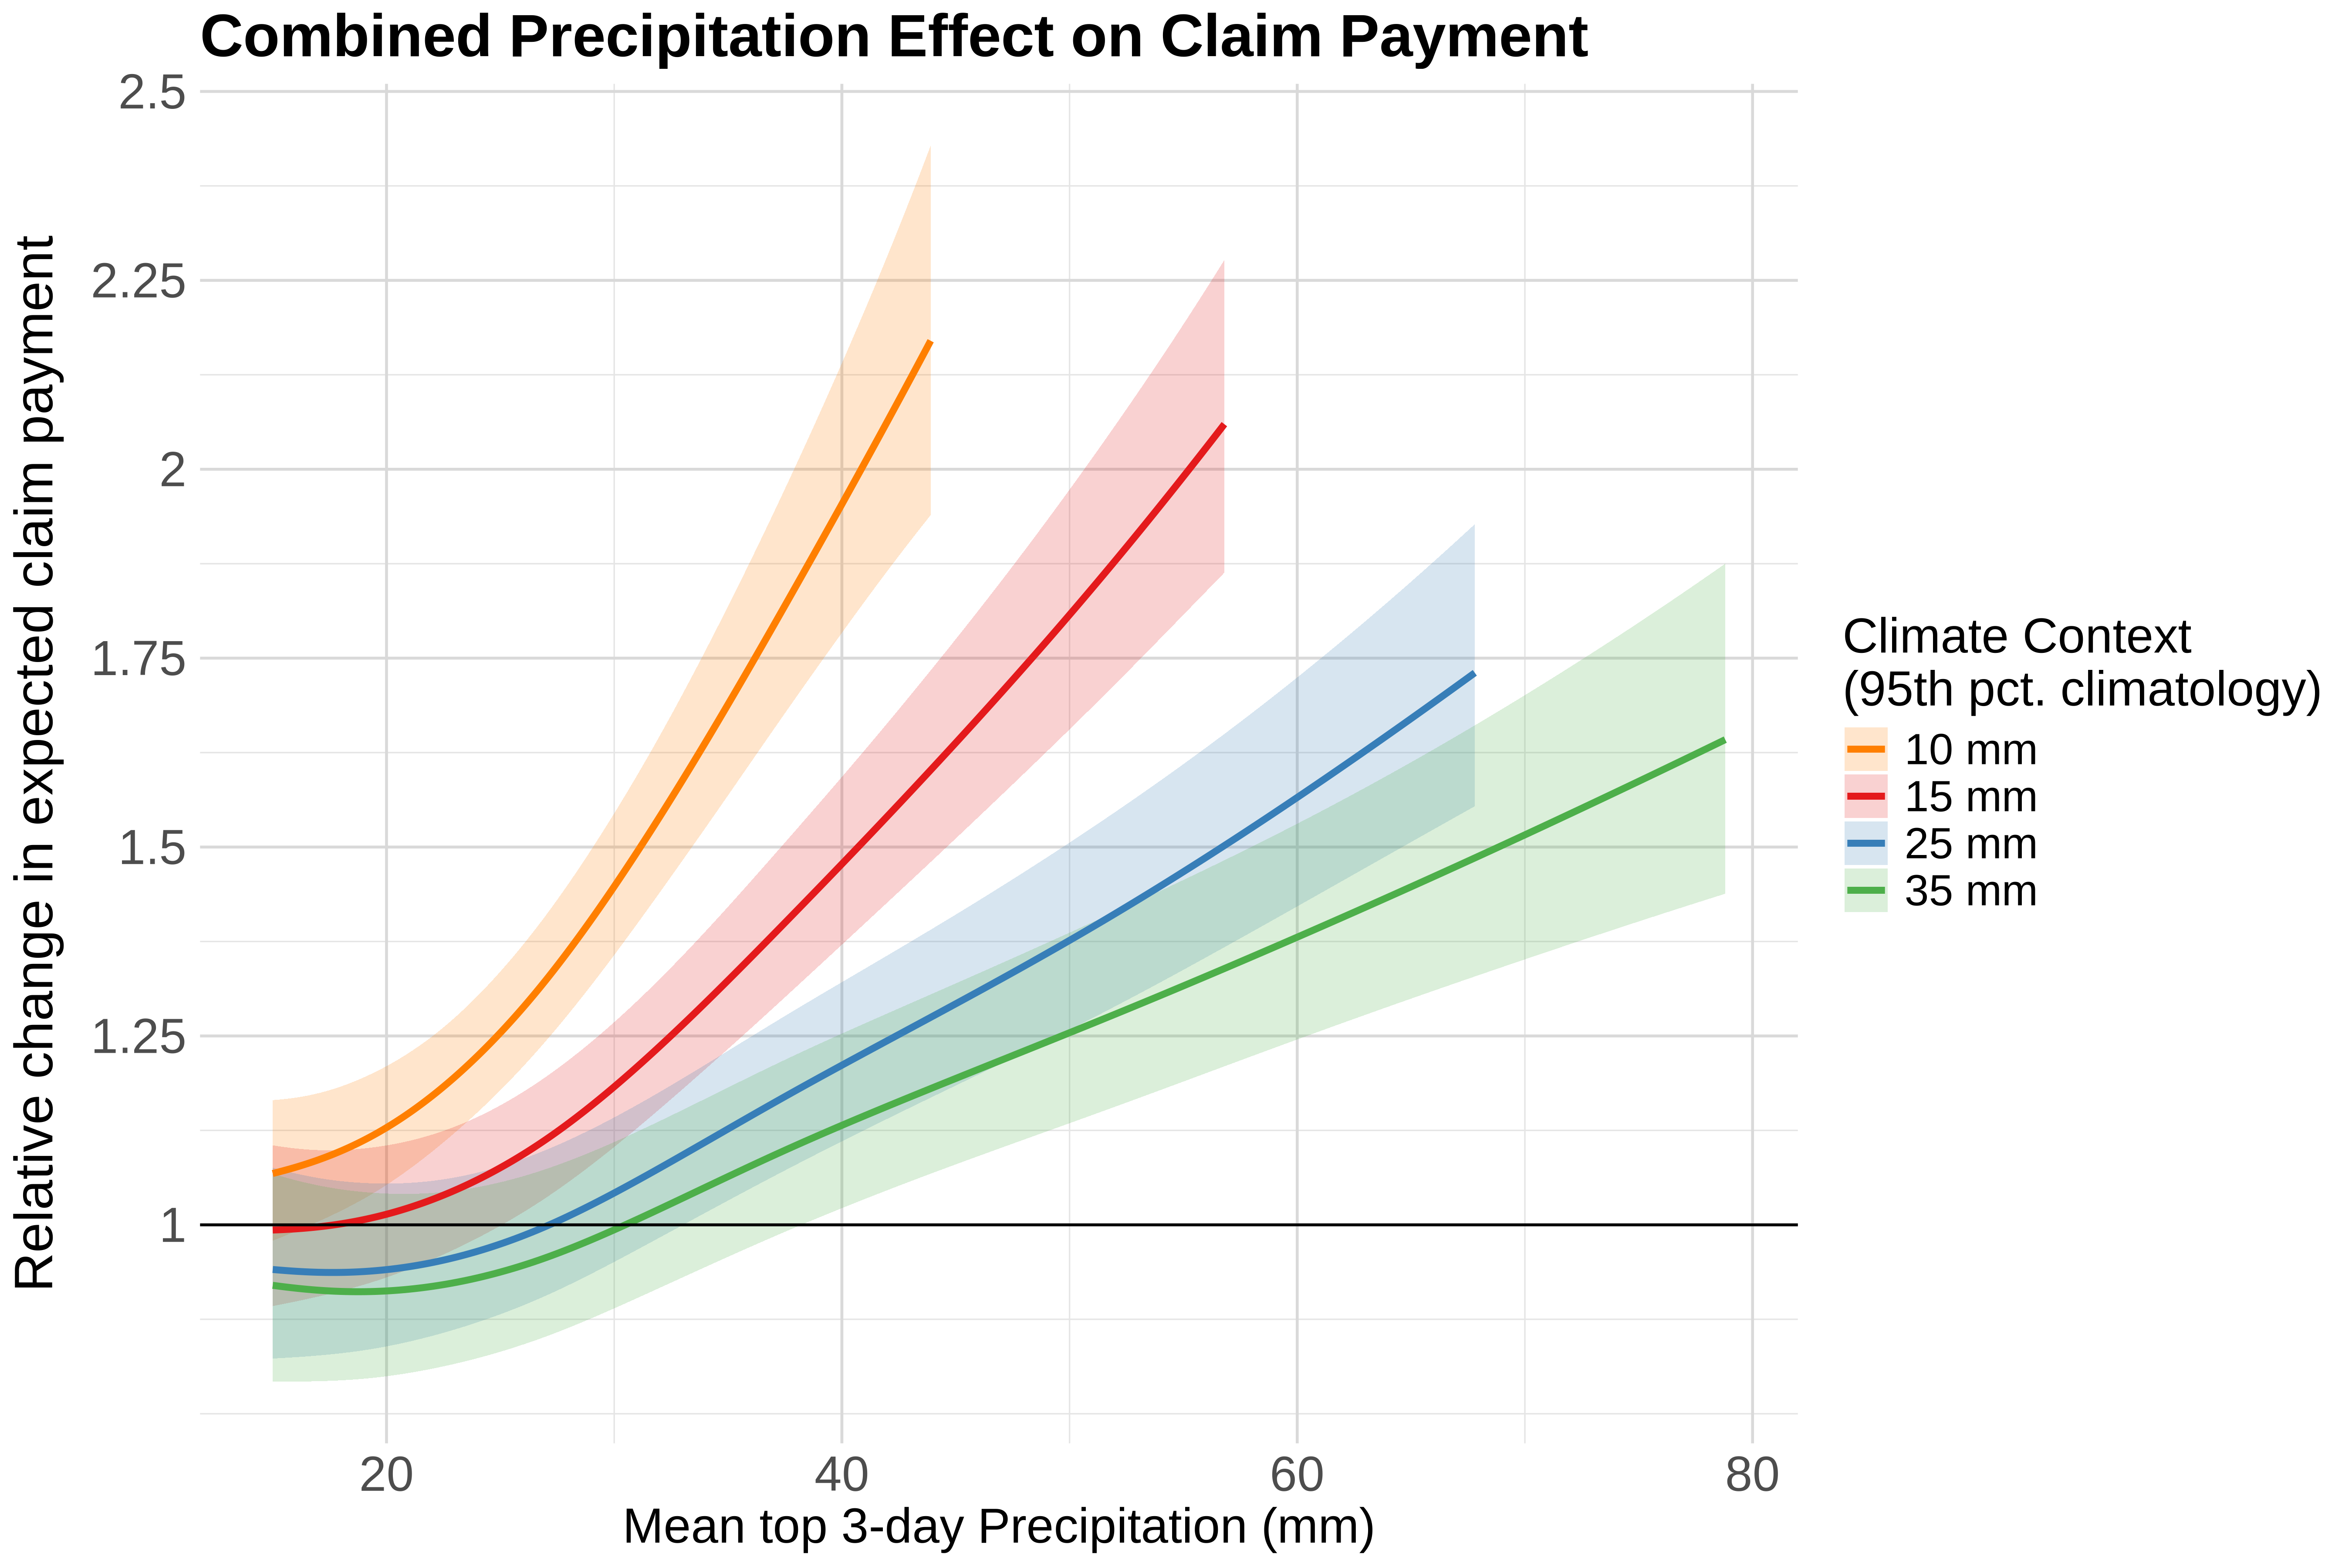
\includegraphics[width=\textwidth,height=0.75\textheight,keepaspectratio,trim={0
  0 0 26},clip]{
  images/model_effects/claim_size_combined_precipitation_effect_presentation_version.png}
\end{frame}
